
\begin{figure}
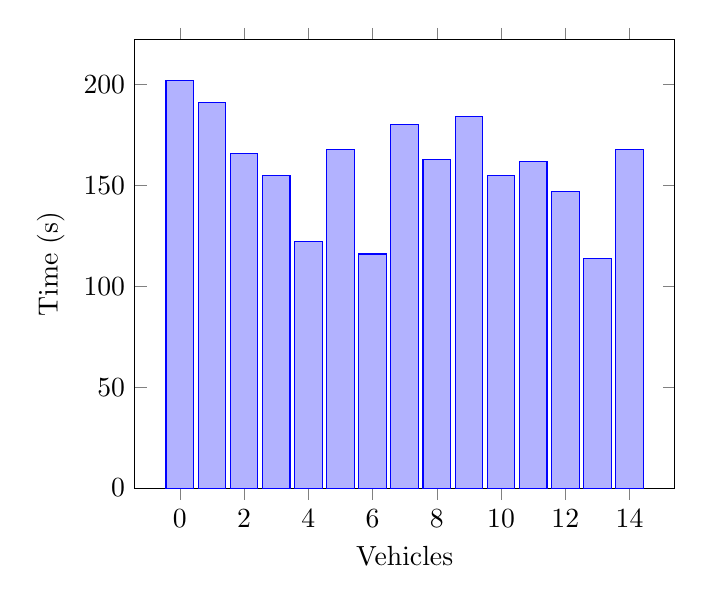
\begin{tikzpicture}
\begin{axis}[
legend style={anchor=west},
xlabel=Vehicles,
ylabel=Time (s),
ymin=0,
ybar,
]
\addplot coordinates {
(0, 202)
(1, 191)
(2, 166)
(3, 155)
(4, 122)
(5, 168)
(6, 116)
(7, 180)
(8, 163)
(9, 184)
(10, 155)
(11, 162)
(12, 147)
(13, 114)
(14, 168)
};

\end{axis}
\end{tikzpicture}
\label{tik:100:21_V, 20_V, 17_N, 15_S, 15_S.-30, 13_N, 13_N.-40, 11_N, 8_N, 7_N, 7_N.-60, 5_N, 4_N, 4_N.-60, 2_V}
\caption{100 percent diving with GSC on route $21_V, 20_V, 17_N, 15_S, 15_S.-30, 13_N, 13_N.-40, 11_N, 8_N, 7_N, 7_N.-60, 5_N, 4_N, 4_N.-60, 2_V$}
\end{figure}
